
\section*{Simulation}
\subsection*{Why Simulate}
To test the system it is much better to simulate the given system instead of doing testing on the real system. That is because then one can do testing without destroying expensive equipment and if multiple people are working on the same project everyone can do simulation test on the system without waiting in turn. It is also easier to perform testing of control algorithms without any disturbances and noise. 

\subsection*{ROS - Robot Operating System}
ROS is not really an operating system as its names states. On their own website ROS is described as a flexible framework for writing robot software. ROS has a collection of libraries, tools, and conventions that are meant to simplify the complex proccess of creating a robust and a good robot software. Tasks that are very simple for us humans will be very complex and hard for a robot. ROS was created in the thought of that everone with knowledge of different robotics aspects can contribute to ROS and at the same time make use of other ressources others have made. In such ways ROS is always in development and encourage groups to collaborate to make ROS better and better. 


\subsection*{RVIZ}
Rviz or ROS visualization, is one the packagages that can be installed to ROS. It is used for 3D visualization gathered from sensor data from the real system or state data from a simulation environment. Rviz is a very good tool to visualize the current state of the robot. If the plan is to use a vision system Rviz is very good to use to see what the robot sees and therefore makes the debugging even easier. 


%For simulation and visualization in ROS, Rviz and Gazebo are used. Gazebo is a simulation environment with a good physics engine which can be used to simulate and test different control algorithms. Rviz is just a visualization tool to visualize the robot configuration and is great to use along with control of actual hardware. 



\begin{figure}[htbp]
  \centering
  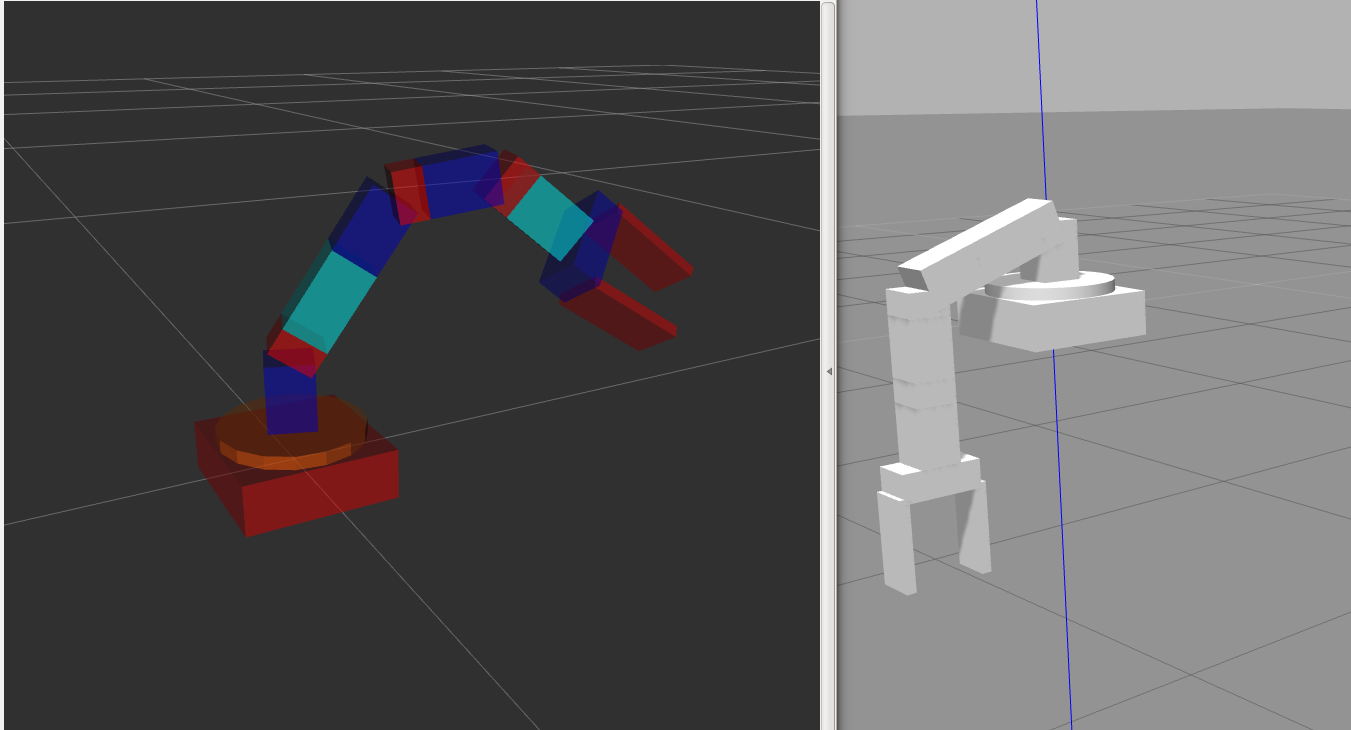
\includegraphics[width=.9\textwidth]{img/test.png}
  \caption{Manipulators visualized in Rviz and Gazebo, respectively}
  \label{fig:robot}
\end{figure}


\section*{Coding}
All the code can be found at this Github repository: \href{https://github.com/Aarskog/robotarm}{\underline{rotbotarm}}


\subsection*{Unified Robot Description Format (URDF)}
So far the model of the manipulator has been done using a Unified Robot Description Format (URDF) file. The syntax is very easy to understand. In \figref{fig:urdf_code_example} some code for the manipulator is given. This code decribes the mounting plates on the motors where the nect link can be mounted on. 
This particular code is a macro which means that it can be reused later in the code such that repeated code is avoided. The first part is the visuals for the plate. The mounting plate is illustrated as a box where length, width and height are specified. The next is collision which states the physical boundaries of the object. And the last is inertia where random inertia values are selected because Gazebo will not accept macroed values.


\begin{figure}[htbp]
  \centering
  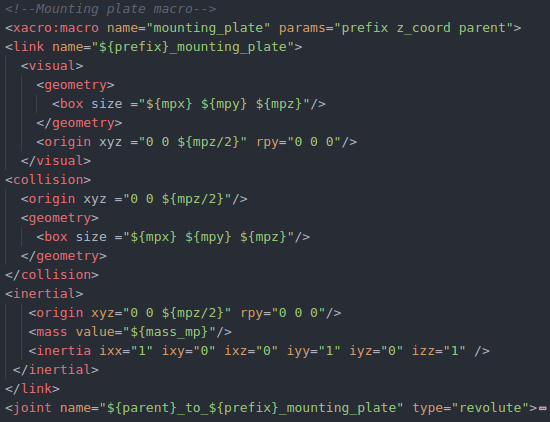
\includegraphics[width=.7\textwidth]{img/urdf_code_example.png}
  \caption{URDF-code example}
  \label{fig:urdf_code_example}
\end{figure}




\subsection*{YAML-file}
In the project, the joints.yaml file is the configuration file that states the torque controller for each joint. As per now a PID controller is used for each joint. This is based on a SISO system for each joint. The dynamic equations of the manipulator is in fact a complex nonlinear and multivariable system. 

\subsection*{Launch files}
The launch files are used for starting up Gazebo,Rviz and the different nodes. It is also used to place the robot model into the simulation environment. The controller nodes are launched form control.launch.





\subsection*{Python}
As per now a single python script is used for control of the manipulator. The task of the script is to listen to the Gazebo topic wich publishes the joint variables. 


\section*{Path planning}


\section*{Trajectory planning}
The trajectory planner decides the joint velocites and accelerations while traversing the path. 
\subsection*{Inverse kinematics}


